\documentclass[a4paper,norsk]{article}
\usepackage{preamble}

\begin{document}
\maketitle
\section*{Taylor-Green Vortex}

\section*{Abstract}

\section*{Physical problem}
The Taylor-Green vortex is a unsteady flow were we observe the flow of a decaying
vortex. This flow has an exact solution for the incrompessible Navier-Stokes equation in 2D, while for the 3D
case there are several numerical results for comparison.
Assuming the fluid is incompressible, the exact solution for velocity and pressure are given as ($t=0$)

\begin{align}
u(x,y,t) = (V_{0} cos(\pi x)sin(\pi y) e^{-2 t \nu \pi^{2} }, \hspace{2mm} V_{0}cos(\pi y)sin(\pi x) e^{-2 t \nu \pi^2} ) \\
p(x,y,t) = -0.25(cos(2\pi x) + cos(2 \pi y) ) e^{-4 t \nu \pi^2}
\end{align}


For the 3D case we will consider the kinetic energy $E_k$ and kinetic energy dissipation rate $\epsilon$  for the system. These quantities are
explored thoroughly by other authors, and will be used as comparison. The initial field set up in the 3D Taylor-Green vortex is defined as

\begin{align}
u(x,y,z) = ( V_{0}sin(\frac{x}{L}) cos(\frac{y}{L}) cos(\frac{z}{L}), \hspace{2mm}-V_{0}cos(\frac{x}{L})sin(\frac{y}{L})cos(\frac{z}{L}), \hspace{2mm} 0 )\\
p(x,y,z) = \rho_{0} + \frac{\rho_0 V_0^2}{16}(cos(\frac{2x}{L}) + cos(\frac{2y}{L}))(cos(\frac{2z}{L}) + 2)
\end{align}

Exploring the incompressible flow condition we define $\rho_0 = \rho$, and for simplicity we let $V_0 = 1$

\section*{Governing Equation and Computations}
The incompressible Naiver-Stokes equation describes the flow motion, from the principles of conservation of momentum
and continuum.

\begin{align}
&\frac{\partial \textbf{v}}{\partial t} + \textbf{v} \cdot \nabla \textbf{v} =
-\nabla p + \nu \nabla^2 \textbf{v} \\
&\nabla \cdot \textbf{v} = 0
\end{align}

There is a open sea full of different approaches to solve this non-linear equation. We will for this
time explore Chorins method, and the incremental pressure correction scheme (\textit{IPCS}).

We will use the FEniCS project, a open-source PDE solver using the finite element method approach.
As verification of our schemes, the known analytical solution for the 2D Taylor-Green Vortex will be used as comparison.
Finally we will move on to the 3D Taylor-Green vortex, using ... as reference.

The Reynolds number, discovered Osborne Reynolds as the relation between inertial and viscous forces, is defined
as
\begin{align}
Re = \frac{\rho V_{0} L}{\mu} = \frac{V_{0} L}{\nu}
\end{align}
Where $\nu$ denotes the kinematic viscosity, while $U_{0}$ and \textit{D} is some characteristic velocity and lenght.

We define the kinetic energy as $E_k = \frac{1}{2}||u||^2_{L^2}$, and the kinetic energy dissipation rate $\epsilon = \frac{-d E_k}{dt}$

\section*{Setting up 2D problem}

For the 2D case, the computational domain is set as $\Omega \in [-1, 1]^2$. Further on we will set
the flow conditions as \\

\begin{tabular}{l*{6}{c}r}
Physical Quantity              & Value  \\
\hline
Reynolds Number, Re & 1000   \\
Characteristic length, L           & 2     \\
Characteristic velocity, $V_{0}$   & 1     \\
Time step $\Delta t$ 			   & 0.001 \\
End time, T 					   & 1.0
\end{tabular}

Using our analytical solution for time $t = 0$, we set up the initial condition
for the domain $\Omega$

\begin{figure}[h!]
	\centering
	\caption*{Initial velocity field}
	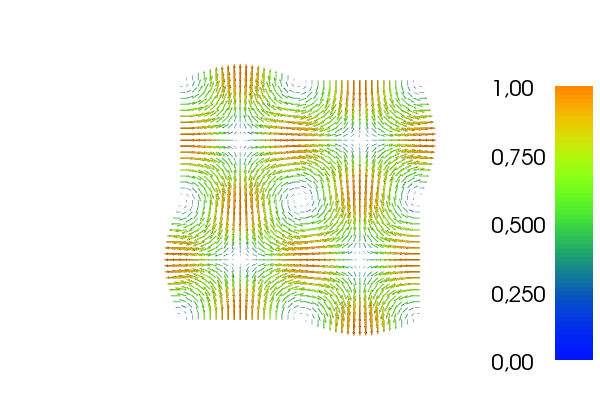
\includegraphics[scale=0.32]{2D/initial.png}
    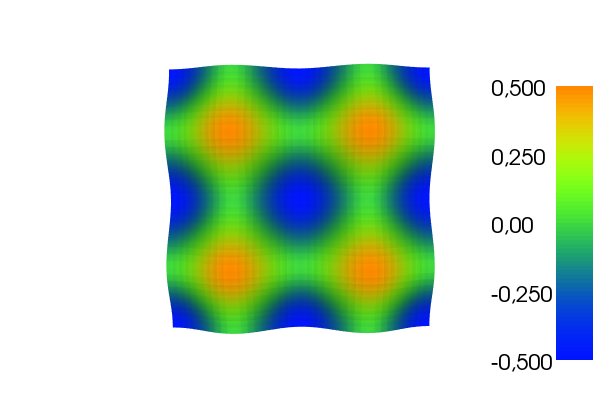
\includegraphics[scale=0.32]{2D/initpress.png}
\end{figure}


\section*{Results}
2D case Oasis Runtime: 3.8886 \\

\begin{lstlisting}
N    dt = 0.1    Runtime    dt = 0.01    Runtime    dt = 0.001    Runtime

8   0.539835    0.164657   0.180778     0.519237   0.178371       4.76148
16   2.04897    0.179117   0.0183534    1.0009     0.0184022      9.40705
32   0.104095    0.400865   0.00130196   2.85381    0.0012364     53.0239
64   0.0210904   1.26767    0.00484368  10.0555     0.000161193  160.618
\end{lstlisting}

Chorin own implementation 7.039

\begin{figure}[h!]
	\centering
	\caption*{Kinetic Energy}
	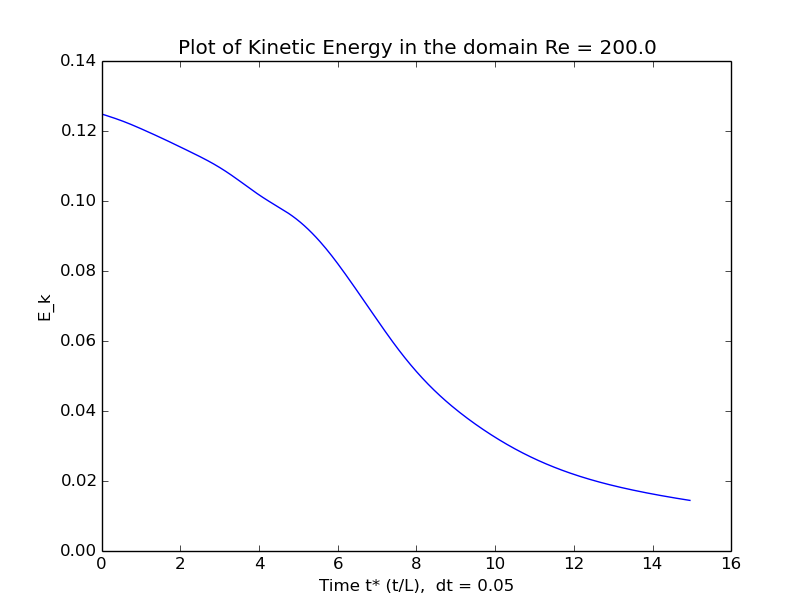
\includegraphics[scale=0.6]{3D/Et.png}
\end{figure}

\begin{figure}[h!]
	\centering
	\caption*{Dissipation Energy}
	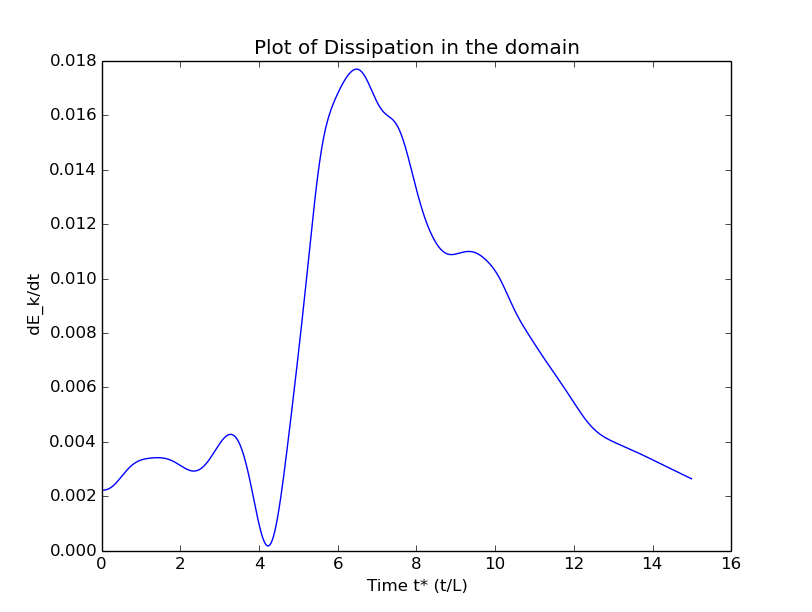
\includegraphics[scale=0.6]{3D/dissi.png}
\end{figure}

\section*{Setting up 3D problem}
The computational domain is defined as a cube with sides of length $2 \pi L$, $-\pi L \leq x,y,z \leq \pi L$

\begin{tabular}{l*{6}{c}r}
Physical Quantity              & Value  \\
\hline
Reynolds Number, Re & 1000   \\
Characteristic length, L           & 1     \\
Characteristic velocity, $V_{0}$   & 1     \\
Time step $\Delta t$ 			   & 0.001 \\
End time, T 					   & 1.0
\end{tabular}

\end{document}
